\documentclass{beamer}
\usepackage[utf8]{inputenc}
\usepackage[T2A]{fontenc}
\usepackage[english, russian]{babel}
%\usepackage[sfdefault, light]{roboto}
\usepackage{epstopdf}
\usepackage[font={footnotesize}, labelfont={footnotesize}]{caption}
\usepackage[font={footnotesize}, labelfont={footnotesize}]{subcaption}
\usepackage{bm}
\usepackage[absolute,overlay]{textpos}
  \setlength{\TPHorizModule}{1mm}
  \setlength{\TPVertModule}{1mm}

\usepackage{tikz}

% Listings
\usepackage{listings}
\definecolor{codegreen}{rgb}{0,0.6,0}
\definecolor{codegray}{rgb}{0.5,0.5,0.5}
\definecolor{codepurple}{rgb}{0.58,0,0.82}
\definecolor{backcolour}{rgb}{0.95,0.95,0.92}
 
\lstdefinestyle{pythonstyle}{
    backgroundcolor=\color{backcolour},   
    commentstyle=\color{codegreen},
    keywordstyle=\color{magenta},
    numberstyle=\tiny\color{codegray},
    stringstyle=\color{codepurple},
    basicstyle=\scriptsize,
    breakatwhitespace=false,         
    breaklines=true,                 
    captionpos=b,                    
    keepspaces=true,                 
    numbers=left,                    
    numbersep=5pt,                  
    showspaces=false,                
    showstringspaces=false,
    showtabs=false,                  
    tabsize=2
}
\lstset{style=pythonstyle, language=Python}

\graphicspath{ {images/} }
\setbeamertemplate{caption}{\raggedright\insertcaption\par}
\def\figurename{}

\title{Базовые модели машинного обучения:\\деревья решений}
\date[\today]{Практика по дисциплине <<Технологии ИИ>>\\\today}
\author[Anton]{Никольская Анастасия Николаевна\\Першин Антон Юрьевич, Ph.D.}

\institute{Программа <<Большие данные и распределенная цифровая платформа>>\\Санкт-Петербургский государственный университет}

\usetheme{tonythequick}

\begin{document}

\begin{frame}
\titlepage
\end{frame}

\setcounter{framenumber}{0}

\section{}

\begin{frame}{Введение}
    \small

    \begin{itemize}
        \item Дерево решений — это метод представления решающих правил в иерархической структуре, состоящей из элементов двух типов — узлов и листьев. 
        \item В узлах находятся решающие правила.
        \item В простейшем случае, в результате проверки правила, множество примеров, попавших в узел, разбивается на два подмножества.
        \item К каждому подмножеству вновь применяется некоторое правило, и процедура рекурсивно повторяется, пока не будет достигнуто некоторое условие остановки алгоритма.
        \item В последнем узле проверка и разбиение не производится и он объявляется листом. 
        \item Лист определяет решение для каждого попавшего в него примера. 
    \end{itemize}
\end{frame}

\begin{frame}{Пример дерева решений}
    \small
    \begin{figure}[H]
        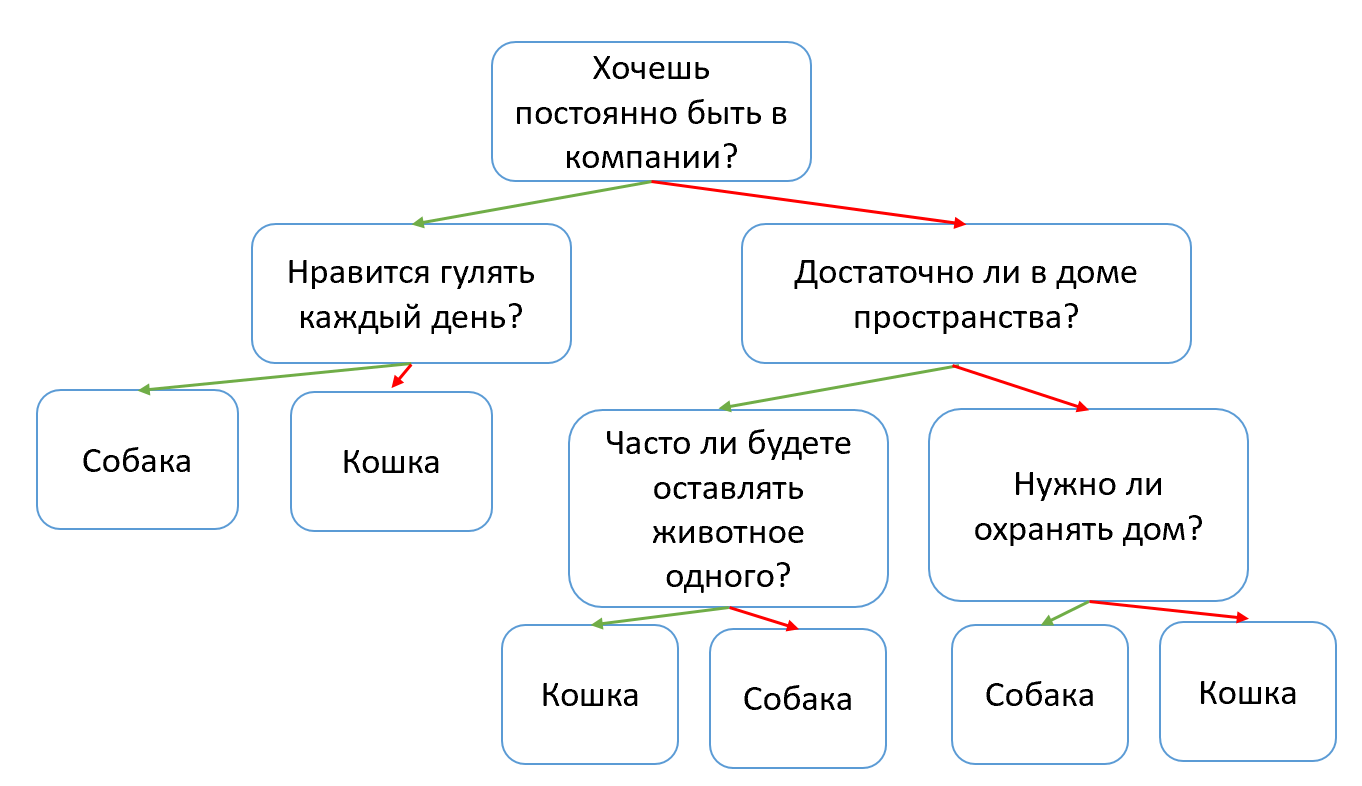
\includegraphics[width=0.8\textwidth]{images/tree.png}
    \end{figure}
\end{frame}


\begin{frame}{Пример дерева решений (2)}
    \small
    \begin{figure}[H]
        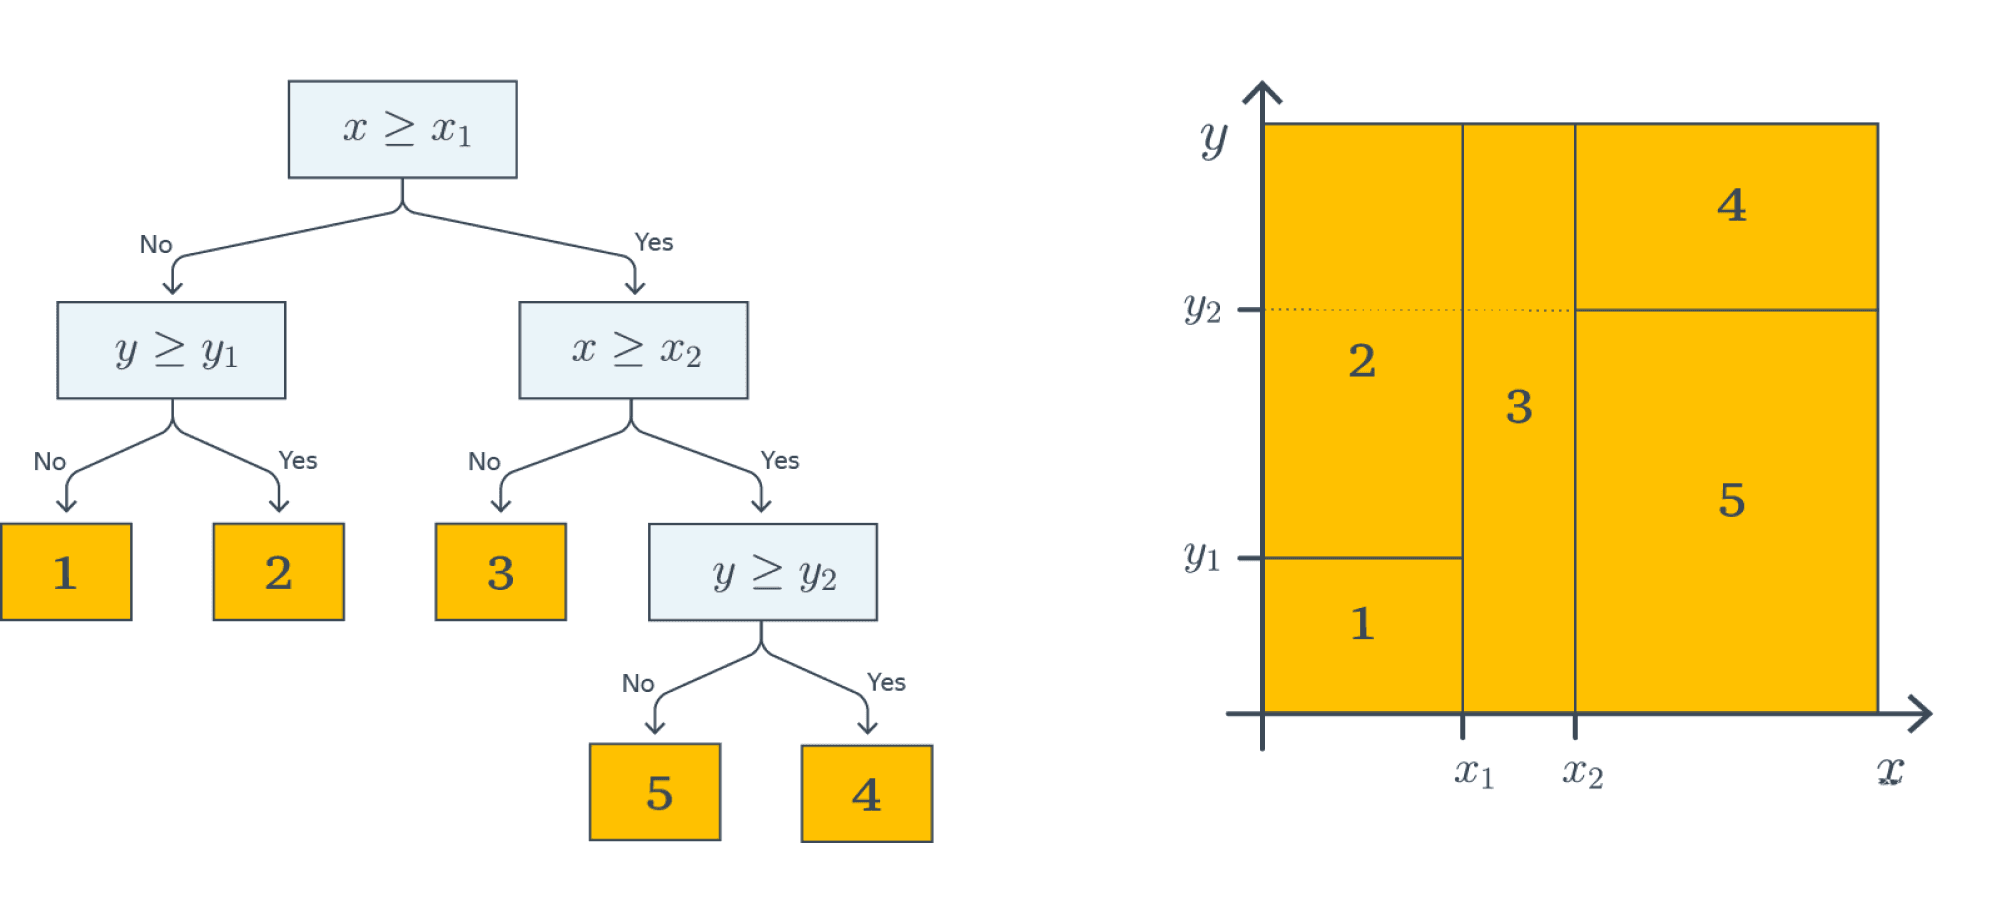
\includegraphics[width=0.8\textwidth]{images/tree_2.png}
    \end{figure}
    \href{https://academy.yandex.ru/handbook/ml/article/reshayushchiye-derevya}{Источник картинки }
\end{frame}


\begin{frame}{Определение решающего дерева}
    \small
    Пусть задано бинарное дерево, в котором:
    \begin{itemize}
         \item каждой внутренней вершине $v$ приписан предикат $Split(v)$ , каждой листовой вершине  приписан прогноз $Ans(v) \in{Y} $, где $Y$ — область значений целевой переменной
        \item В ходе предсказания осуществляется проход по этому дереву к некоторому листу. Для каждого примера движение начинается из корня. 
        \item В очередной внутренней вершине проход продолжится вправо, если $Split(v)=1$, и влево, если $Split(v)=0$. Проход продолжается до момента, пока не будет достигнут некоторый лист и будет получен $Ans(v)$.
    \end{itemize}
    
\end{frame}

\begin{frame}{Свойства решающего дерева}
    \small
    Пусть задано бинарное дерево, в котором:
    \begin{itemize}
         \item Выученная функция является кусочно-постоянной (что из этого следует?)
        \item Дерево решений не может экстраполировать зависимости за границы области значений обучающей выборки
        \item Дерево решений способно идеально приблизить обучающую выборку и ничего не выучить, если выродится (в каждый лист попадет один пример)
    \end{itemize}
    
\end{frame}


\begin{frame}{Жадный алгоритм построения дерева}
    \small
    \begin{itemize}
        \item Создаём вершину $v$
        \item Если выполнен критерий остановки $Stop(S_m)$, останавливаемся, объявляем эту вершину листом и присваиваем ей ответ $Ans(S_m)$
        \item Иначе: находим предикат $Split(S_m)$ , обеспечивающий наилучшее разбиение выборки по некоторому критерию.
        \item Повторяем процедуру для $S_{m_i}$ и $S_{m_j}$ до достижения критерия остановки.
        \item В разных алгоритмах применяются разные эвристики для ``ранней остановки'' или ``отсечения'', чтобы избежать построения переобученного дерева.
    \end{itemize}
\end{frame}

\begin{frame}{Жадный алгоритм построения дерева (2) }
    \small

    \begin{itemize}
        \item  $Ans(S_m)$ в случае задачи классификации — метка самого частого класса или оценка дискретного распределения вероятностей классов для объектов, попавших в этот лист; в случае задачи регрессии — среднее, медиана или другая статистика;
        \item Критерий остановки  — функция, которая решает, нужно ли продолжать ветвление или пора остановиться. Это может быть какое-то тривиальное правило, равенство или близость энтропии нулю или достижение максимального числа итераций.
        \item Строгой теории, которая бы связывала оптимальность выбора разных вариантов критериев разбиения и разных метрик классификации и регрессии, в общем случае не существует.
    \end{itemize}
\end{frame}

\begin{frame}{Энтропия}
    \small

    \begin{itemize}
        \item Энтропия Шеннона определяется для системы с $N$ возможными состояниями как:
        \begin{equation}
          H = - \sum_{i=1}^N p_i \log_2 {p_i},
        \end{equation}
        где $p_i$ – вероятности нахождения системы в $i$-ом состоянии
        \item Энтропия может рассматриваться как мера неоднородности подмножества по представленным в нём классам
        \item Энтропия максимальна при равномерном распределении классов и равна 0, если подмножество содержит только один класс
    \end{itemize}
\end{frame}

\begin{frame}{Информационный подход к разбиению}
    \small

    \begin{itemize}
        \item Лучшим атрибутом разбиения будет тот, который обеспечит максимальное снижение энтропии результирующего подмножества относительно родительского
        \item Тогда лучшим критерием будет тот, который обеспечит максимальный прирост информации ( $Info = -S$):
        \begin{equation}
          Gain(A) = Info(S) - Info(S_A) = Info(S) - \sum_{i=1}^q \frac{N_{i}}{ N } Info(S_i),
        \end{equation}
        где $S$ -- множество до разбиения, $S_A$ -- разбиение множества по атрибуту $A$ на $q$ групп, $N_i = |S_i|$ и $N = |S|$.
        \item Т.о. задача выбора атрибута разбиения в узле заключается в максимизации величины $Gain(A)$
    \end{itemize}
\end{frame}


\begin{frame}{Статистический подход}
    \small

    \begin{itemize}
        \item В основе статистического подхода лежит использование неопределенности Джини
        \item Он показывает — насколько часто случайно выбранный пример обучающего множества будет распознан неправильно
        \item Т.о он показывает расстояние между целевым распределением и распределением предсказаний
        \item  Неопределенность Джини можно рассчитать по формуле:
        \begin{equation}
          Gini(Q) = \sum_{i=1, N} p_i (1 - p_i) = 1 - \sum_{i=1, N}{p_i}^2,
        \end{equation}
        где $S$ - множество до разбиения, $S_A$ - разбиение множества по атрибуту $A$
        \item Т.о. максимизируется число объектов одного класса, попавших в поддерево
        \item Hеопределенность Джини и прирост информации работают почти одинаково
    \end{itemize}
\end{frame}



\begin{frame}{ Неоптимальность критериев разбиения }
    \small
    \begin{itemize}
        \item  Жадный алгоритм не даст оптимального решения задачи XOR.
        \item Иногда оптимальное с точки зрения выбранной метрики дерево получается с критерием ветвления, построенным по другой метрике
    \end{itemize}
    \begin{figure}[H]
        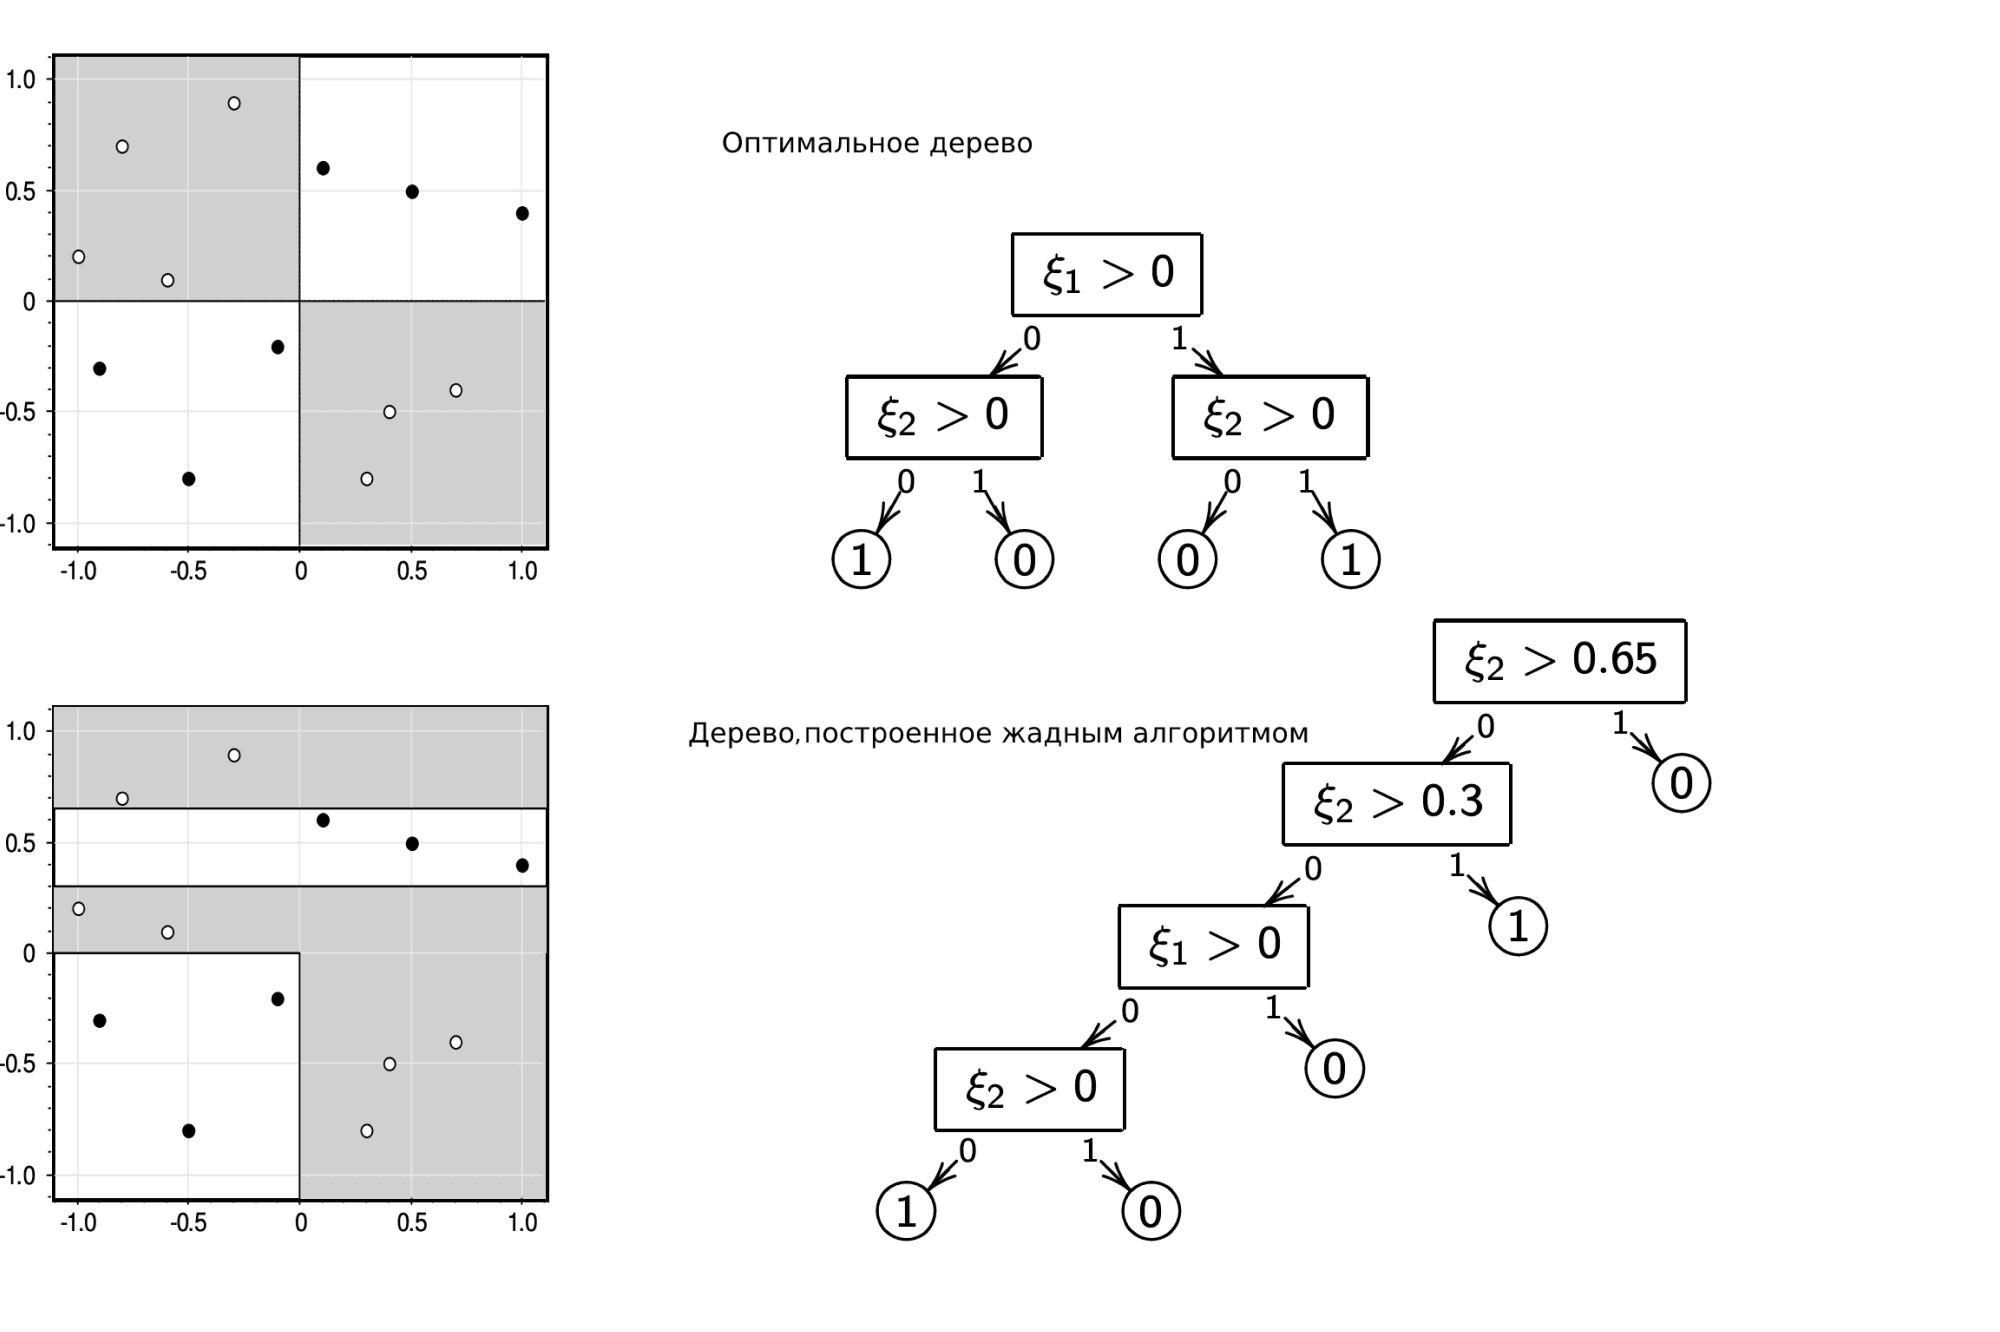
\includegraphics[width=0.7\textwidth]{images/xor.png}
    \end{figure}
    \href{http://www.machinelearning.ru/wiki/images/archive/9/97/20140227072517!Voron-ML-Logic-slides.pdf}{Источник картинки }
\end{frame}


\begin{frame}{ Категориальные признаки}
    \small
        
    \begin{itemize}
       \item Если признак принимает значения $C \in \{ c1...c_m\}$, то простой перебор даст $2^{m-1} - 1$ сплитов
       \item Перебирать их слишком долго, и часто их пытаются упорядочить
       \item Для бинарной задачи можно упорядочить категории по доле примеров класса 1 со значением $c_i$
       \item Для регрессии - по среднему значению таргета
    \end{itemize}
\end{frame}


\begin{frame}{ Регуляризация}
    \small
    Чтобы дерево не переобучалось, ветвление обычно останавливают по одному из следующих критериев:
    \begin{itemize}
       \item Ограничение по максимальной глубине дерева
       \item Ограничение на минимальное количество объектов в листе
       \item Ограничение на максимальное количество листьев в дереве
       \item Требование, чтобы функционал качества при делении текущей подвыборки на две улучшался не менее чем на $S$ процентов
    \end{itemize}
\end{frame}

\end{document}
